% !TeX spellcheck = en_US
\newpage
\section{Anomalies}
Anomalies are points that escape the models prediction capabilities. Hence, a model for anomaly detection should focus on the opposite of what's been predicted to be normal.

\begin{example}
	An example application is when discovering anomalous or rare geological properties for resource monitoring and extraction.
\end{example}

\subsection{Classical}
\subsubsection{Z-score}
The Z-score is a common measure of anomalies in statistical studies.
\begin{equation}
	z = \frac{(x - \mu)}{\sigma}
\end{equation}
Where $\mu$ is the \textit{mean} and $\sigma$ the \textit{standard deviation}.
\begin{center}
	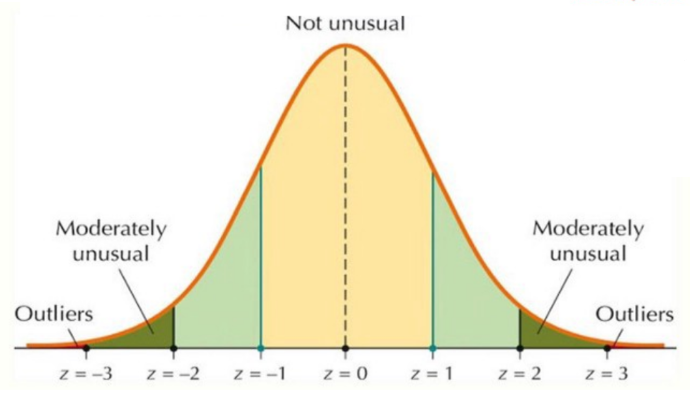
\includegraphics[scale=0.3]{zscore}
\end{center}
Points can be considered outliers if their z-score is above a certain threshold, usually $\lvert z \rvert > 3$.

\begin{observation}
	When input feature are correlated (\textbf{multivariate data}), z-score of individual features cannot properly detect outliers.
\end{observation}

\subsubsection{Mahalanobis Distance}
The Mahalanobis Distance is the generalization of the concept of the z-score. It defines how many standard deviations the model is away from the center of the data, taking into account \textbf{correlations}. \\\\
The Mahalanobis Distance of a point $x \in \mathbb{R}^d$ to a reference distribution of mean $\mu \in \mathbb{R}^d$ and covariance $\Sigma\in \mathbb{R}^{d\times d}$ is defined as:
\begin{equation}
	z=\sqrt{(x-\mu)^T \Sigma^{-1}(x-\mu)}
\end{equation}
\begin{center}
	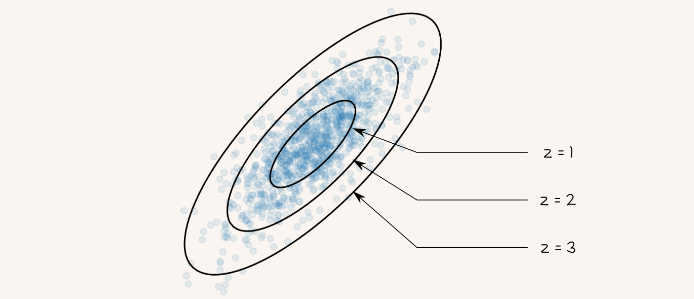
\includegraphics[scale=0.3]{md}
\end{center}

We can relate the distance to the z-score computed in PCA space by the formula
\begin{equation}
	z = \sqrt{\sum_{j=1}^{d}(x_{\text{PCA}-j})^2}
\end{equation}

\paragraph{Limits} The main problem is that in high dimensions the matrix $\Sigma^{-1}$ tends to get \textbf{uncontrollably large} due to the correlations that arise from the limited data. This instability can be addressed by adding a small diagonal term to the covariance matrix, making the anomaly score more robust.
\begin{equation}
	\Sigma \leftarrow \Sigma+\epsilon I
\end{equation}
Furthermore, in presence of \textbf{skewed non-Gaussian} distribution, the Mahalanobis Distance does not describe well data.

\subsection{Boundary-Based}
The idea behind this method is to learn a geometrical object that encloses most of the data but the outliers. E.g. hyper sphere or polytope.
\begin{equation}
	\mathcal{O}(S,\mathbf{c}) = \{\mathbf{x} \in \mathbb{R}^d : h(\mathbf{x}, \mathbf{c}) \leq S\}
\end{equation}
Then we have to find a minimum enclosing object:
\begin{equation}
	\min_{S, \mathbf{c}, \mathbf{\varepsilon}} S+C\sum_{i=1}^{N}\varepsilon_i \qquad\qquad \forall_{i=1}^N : h(\mathbf{x}_i; \mathbf{c}) \leq S + \varepsilon_i \qquad\forall_{i=1}^N : 0 \leq \varepsilon_i
\end{equation}
Optimization problem with inequality constraints, like this one, can be studied within KKT conditions.

\subsubsection{KKT Conditions}
\begin{definition}[KKT Conditions]
	Given an optimization problem in the following form
	\begin{equation*}
		\min_\theta f(\mathbf{\theta}) \qquad\qquad \forall_{i=1}^M : g_i(\mathbf{\theta}) \leq 0
	\end{equation*}
	e defined the Lagrangian function
	\begin{equation*}
		\mathcal{L}(\mathbf{\theta}, \mathbf{\lambda}) = F(\mathbf{\theta}) + \sum_{i=1}^{M} \lambda_i g_i(\mathbf{\theta})
	\end{equation*}
	If $\mathbf{\theta}^*$ is a solution of the optimization problem, and the latter satisfies some regularity conditions (e.g. objective convex, all constraint convex and existence of $\mathbf{\theta}$ that satisfies them with strict inequalities), then exists a constant vector $\mathbf{\lambda}$ such that the solution satisfies:
	\begin{itemize}
		\item \textbf{Stationarity}
		\begin{equation}
			\nabla_\mathbf{\theta} \mathcal{L}(\mathbf{\theta^*}, \mathbf{\lambda}) = 0
		\end{equation}
		\item \textbf{Primal feasibility}
		\begin{equation}
			\forall_{i=1}^M : g_i(\mathbf{\theta^*}) \leq 0
		\end{equation}
		\item \textbf{Dual feasibility}
		\begin{equation}
			\forall_{i=1}^M:\lambda_i \geq 0
		\end{equation}
		\item \textbf{Complementary slackness}
		\begin{equation}
			\forall_{i=1}^M: \lambda_i g_i(\mathbf{\theta^*}) = 0
		\end{equation}
	\end{itemize}
\end{definition}

KKT conditions provide a set of equation with a solution $\mathbf{\theta^*}$ needs to satisfy. Usually they cannot be solved analytically and thus optimization is needed. There are two approaches:
\begin{itemize}
	\item \textbf{Primal}: solve the optimization problem
	\begin{equation}
		\min_\mathbf{\theta} f(\mathbf{\theta}) \qquad\qquad \forall_{i=1}^M: g_i(\mathbf{\theta}) \leq 0
	\end{equation}
	\item \textbf{Lagrange Dual}: the idea is to penalize constraint violations directly into the objective
	\begin{equation}
		\max_{\mathbf{\lambda}\succeq 0} \inf_\mathbf{\theta} \big\{f(\mathbf{\theta}) + \sum_{i=1}^{M} \lambda_i g_i(\mathbf{\theta})\big\}
	\end{equation}
	Then the primal parameters $\mathbf{\theta^*}$ can be recovered from the dual solution $\mathbf{\lambda}^*$ using KKT conditions.
\end{itemize}

\subsection{SVDD}
Support Vector Data Description requires the building of a hyper sphere
\begin{equation}
	\mathcal{H} = \{\mathbf{x} \in \mathbb{R}^d: \lvert\lvert \mathbf{c} - \mathbf{x} \rvert\rvert^2 = S\}
\end{equation}
with parameters $(\mathbf{c}, S)$ where $S=R^2$ is a variable modeling the square radius. They are chosen in a way that encloses most data points and has minimum radius.\\
Points should be included in $\mathcal{H}$, however to account fo anomalies, one allows points to be outside with a \textbf{penalty} $\varepsilon_i$.\\
The problem can be stated as the convex optimization problem
\begin{equation}
	\min_{S, \mathbf{c}, \mathbf{\varepsilon}} S + C \sum_{i=1}^N \varepsilon_i \qquad\qquad \forall_{i=1}^N: \lvert\lvert \mathbf{x}_i - \mathbf{c} \rvert\rvert ^ 2 \leq S + \varepsilon_i \qquad \forall_{i=1}^N : \varepsilon_i \leq 0
\end{equation} 
This has $1+d+N$ parameters, so it may not scale well with high-dimensional data. Therefore we can derive the \textbf{dual} optimization problem through KKT, which has only N parameters and linear constraints
\begin{equation}
	\max_{\mathbf{\alpha}}\sum_{i=1}^N \alpha_i \lvert\lvert \mathbf{x}_i \rvert\rvert ^ 2 - \sum_{i=1}^{N} \sum_{j=1}^{N} \alpha_i \alpha_j \mathbf{x}_i^T \mathbf{x}_j \qquad\qquad \sum_{i=1}^N \alpha_i = 1 \qquad \forall_{i=1}^N: 0 \leq \alpha_i \leq C
\end{equation}
\begin{wrapfigure}[10]{r}{4cm}
	\begin{center}
		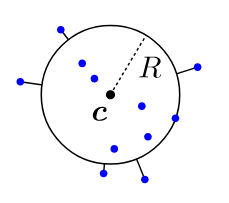
\includegraphics[width=4cm]{svdd}
	\end{center}
\end{wrapfigure}
From the dual we can get:
\begin{itemize}
	\item \textbf{Center}, a weighted average of points, with the \textit{stationary condition}
	\begin{equation}
		\mathbf{c} = \sum_{i=1}^{N} \alpha_i \mathbf{x}_i
	\end{equation}
	\item \textbf{Radius}, with the \textit{complementary slack}:
	\begin{align*}
		& \alpha_i \cdot (\lvert\lvert \mathbf{x}_i - \mathbf{c} \rvert\rvert^2 - S - \varepsilon_i) = 0\\
		& (C - \alpha_i) \cdot (-\varepsilon_i) = 0
	\end{align*}
	which yields for any point $i$ satisfying $0 < \alpha_i < C$ the equation $S=\lvert\lvert \mathbf{c} - \mathbf{x}_i \rvert\rvert^2$, or rather
	\begin{equation}
		R = \lvert\lvert \mathbf{c} - \mathbf{x}_i \rvert\rvert
	\end{equation}
\end{itemize}

\begin{observation}
	We can infer that any point inside the hyper sphere must have $\alpha_i = 0$, therefore the hyper sphere is only determined by points at the border of the distribution.
\end{observation}

\subsubsection{Comparison}
Compared to the Mahalanobis Distance, the SVDD model is more robust to the \textbf{skew} data, due to its ability to focus mainly on the border of the distribution. At the same time, for the same reason, it's more \textbf{"blurry"}

\subsubsection{Improvement}
The decision boundary of SVDD is greatly distorted by strong \textbf{outliers}, which may be interesting points or artifacts that we want to ignore. \\
To prevent this we need to robustify the model in two steps:
\begin{enumerate}
	\item Rewrite SVDD as the \textbf{constraint-free} optimization problem
	\begin{equation}
		\min_{S, \mathbf{c}, \mathbf{\varepsilon}} S + C \sum_{i=1}^N \underbrace{\max(0, \lvert\lvert \mathbf{x}_i - \mathbf{c}\rvert\rvert^2 - S)}_{\varepsilon(\mathbf{x}_i)}
	\end{equation}
	The added function $\max$ handles the two cases where the point is inside or outside of the hyper sphere. The problem is still convex and we can use gradient descent.
	\item Consider the alternative convex optimization problem
	\begin{equation}
		\min_{S, \mathbf{c}, \mathbf{\varepsilon}} S + C \sum_{i=1}^N \underbrace{\max(0, \lvert\lvert \mathbf{x}_i - \mathbf{c}\rvert\rvert - S)}_{\varepsilon^{(\text{new})}(\mathbf{x}_i)}
	\end{equation}
	Like the first step, the penalty $\varepsilon$ is triggered when the data point leaves the hyper sphere. However it grows \textbf{linearly} with the distance of the data point from the center. The problem is still convex and we can use gradient descent.
\end{enumerate}